In this section, we describe the mechanisms behind the three components of the Jr. AI Scientist: idea generation, experimentation, and writing. 
First, in \Cref{subsec_prepare}, we describe the necessary preparation.
Next, in \Cref{subsec_idea_generation}, we explain the methods for idea generation. Next, in \Cref{subsec_experiment}, we discuss how agents can execute and manage experiments. Finally, in \Cref{subsec_writing}, we explain the writing process.

\begin{figure*}[t]
    \centering
    \resizebox{\textwidth}{!}{%
    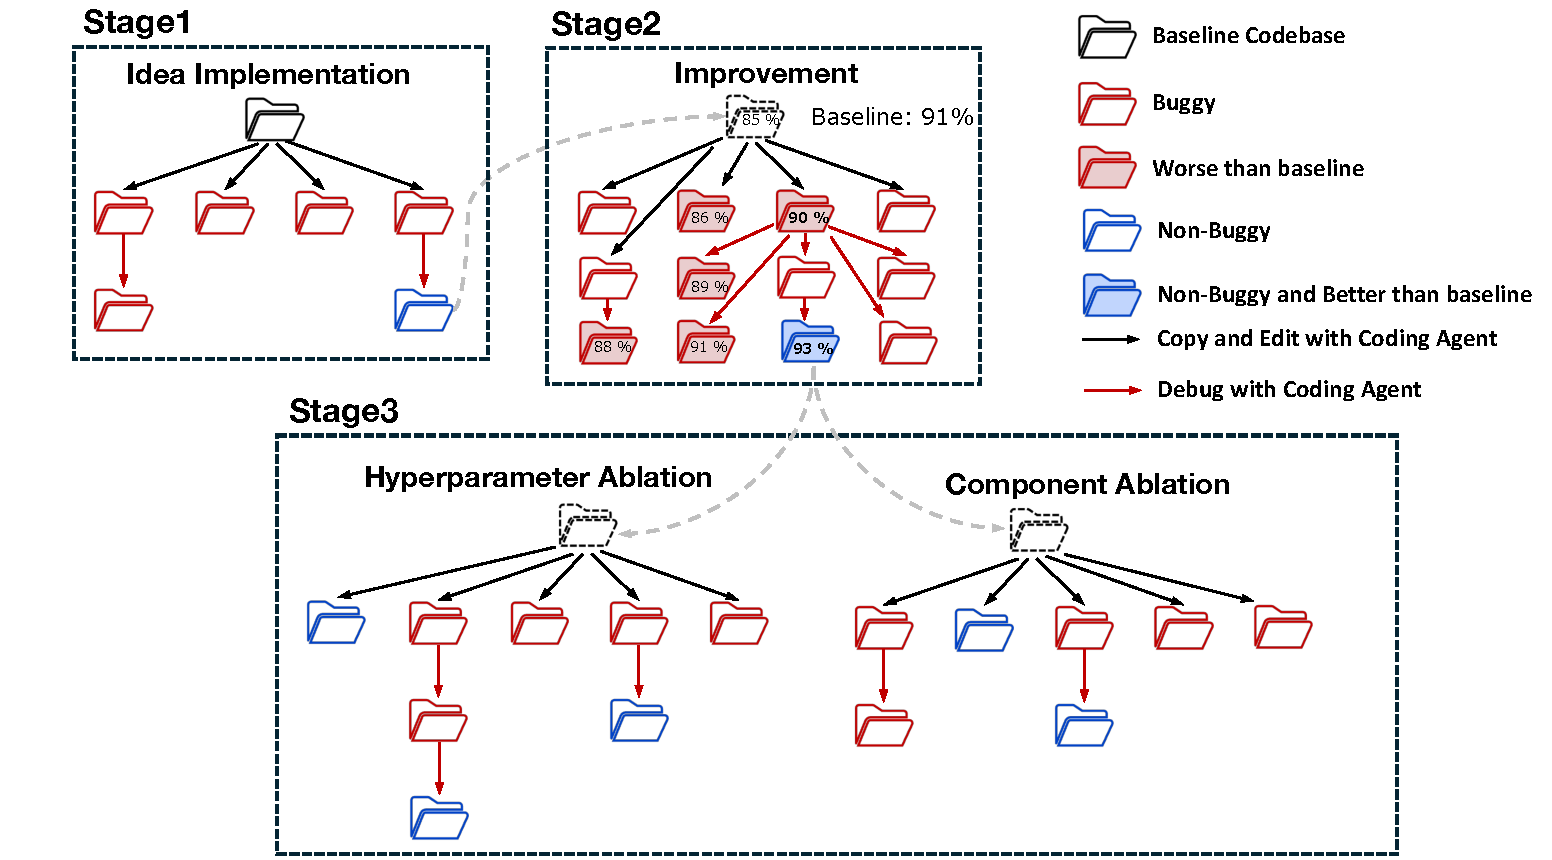
\includegraphics{images/system_workflow.pdf}
    }
    \caption{\textbf{Jr. AI Scientist Workflow for the Experiment Phase.} The workflow consists of three stages.  Through bug management and performance tracking, our system passes the most promising experimental nodes to the next stage.}
    \label{fig:exp_workflow}
\vspace{-2em}
\end{figure*}

\subsection{Preparation: Baseline Paper Selection}
\label{subsec_prepare}
The preparation stage involves selecting a baseline paper, obtaining its LaTeX source files and PDF, and the baseline code. This setup is realistic because many recent publications are released on arXiv with LaTeX sources, and their implementation code is shared on GitHub. While there might be some augment that AI agents should automatically select a baseline and reproduce the code, current reproducibility rates from papers are still limited~\citep{siegel2024core,xiang2025scireplicate,starace2025paperbench}, making complete automation premature. Since our goal is to emulate how a human scientist engages in early-stage research under the guidance of a mentor, we explicitly include this preparatory stage.

When constructing the baseline code, we followed AI Scientist v1~\citep{lu2024ai} and made only minor modifications to the existing implementation so that the experiments could be executed via \texttt{baseline.py} and the results could be visualized via \texttt{plot.py}.
Defining such an experimental entry point facilitated easier management and reproducibility of the execution process in the experimental section.



\subsection{Idea Generation Phase}
\label{subsec_idea_generation}
We provide a baseline paper as text to an LLM (\eg~o4-mini~\citep{o3-o4-mini}) and prompt it to output the limitations of the work. Based on both the baseline paper and the limitations, the LLM is then guided to propose potential research ideas.
Following AI Scientist v2 \citep{yamada2025ai}, the system evaluates the originality of proposed ideas through literature review tools such as Semantic Scholar, which review papers citing the baseline work and papers with similar concepts. If conceptually similar ideas are identified, they are refined; otherwise, they are clearly distinguished from prior work.
These steps define the preliminary research idea. 
\subsection{Experiment Phase}
The Experiment Phase mainly involves implementing and iterating on the implementations through experiments.
It is divided into three stages: Stage 1: Idea Implemention, Stage 2: Iterative Improvement, and Stage 3: Ablation Study. The workflow of each stage is shown in \Cref{fig:exp_workflow}.
We first describe the general procedure for using the coding agent, followed by an explanation of the implementation at each stage.

\label{subsec_experiment}
\subsubsection{Preliminary: Coding Agent Usage}

A powerful coding agent (\eg~Claude Code~\citep{claude_code}) is employed to translate research ideas into concrete implementations.
We provide the coding agent with a working directory that contains the baseline implementations (prepared at \Cref{subsec_prepare}) and give it detailed instructions through input prompts.  
The agent is informed of how to use the main scripts—\texttt{baseline.py}, which serves as the experimental entry point, and \texttt{plot.py}, which visualizes the experimental results.  
We use \texttt{claude-sonnet-4-20250514} within Claude Code (version 1.0.24).

The coding agent is allowed to read and write any files within the working directory.  
For efficient directory exploration, it is permitted to use commands such as \texttt{ls} and \texttt{grep}, while commands that may cause side effects (\eg~\texttt{python} or other execution commands) are not allowed.  
After the agent generates a runnable file (\eg~\texttt{proposed\_method.py} in Stage1), our system mechanically executes the specified command.  
The coding agent is generally given up to 30 turns to complete each assigned task.

\subsubsection{Stage1: Idea Implemention}
The system manages four experimental nodes running in parallel, each responsible for implementing and testing a proposed idea independently.
Within each node, the coding agent receives the baseline code and a research idea, and writes a directly executable script named \texttt{proposed\_method.py}.
Once the coding agent finishes writing the implementation, the system sequentially runs \texttt{proposed\_method.py} and \texttt{plot.py}. 
If a result file is successfully generated, the codebase is marked as Non-Buggy; otherwise, it is labeled as Buggy
If a visualization image is also produced, it is further marked as Non-Plot-Buggy; otherwise, as Plot-Buggy.
Each iteration of this process, coding and execution, is counted as one trial and is repeated until a bug-free implementation is obtained.

As shown in \Cref{fig:exp_workflow}, if any node completes successfully without encountering bugs, its codebase is carried forward to Stage 2. 
During execution, four experimental nodes are selected. If all currently running nodes fail, the system selects the next nodes, either by initializing new nodes from the baseline code or by debugging previously generated buggy codebases.
When debugging buggy codebases, we provide the coding agent with detailed runtime feedback, such as standard output and error messages, to guide iterative debugging until the issue is resolved.
We set this stage to run for 12 iterations.

\subsubsection{Stage2: Iterative Improvement}
Stage 2 focuses on iteratively improving the method implemented in Stage 1 until its performance metrics surpass those of the baseline.
In each trial, the coding agent first proposes an improvement idea to the experimental code, and then applies the modification based on the improved idea.
To avoid overwriting the Stage 1 results, we instruct the coding agent to use a new entry file named \texttt{improved\_proposed\_method.py} as the implementation target.
The system then executes this script, followed by \texttt{plot.py}, to generate results and visualizations in the same manner as Stage 1.

As shown in \Cref{fig:exp_workflow}, for each trial, the experimental codebase is selected probabilistically from either (1) the Stage 1 implementation or (2) the node containing the best-performing implementation observed so far.
Stage 2 ends when a bug-free implementation surpasses the baseline performance.
The resulting code is then passed to Stage 3.
We set this stage to run for 50 iterations.


\subsubsection{Stage3: Ablation Study}
Stage 3 performs ablation studies on the improved method implemented in Stage 2.
In each trial, the system uses an LLM to generate ablation study ideas and then employs the coding agent to implement corresponding scripts based on those ideas.
To encourage higher-quality ablation ideas, we first instruct the coding agent to produce a textual description of the Stage 2 method, which is then provided to the LLM as context for generating more meaningful ablation ideas.
The generated ablation ideas include hyperparameter ablations, which analyze the sensitivity of the method to key hyperparameters, and component-level ablations, which assess the contribution of each component to the overall performance. To avoid overwriting Stage 2's code, we instruct the coding agent to use new entry files named \texttt{hyperparam\_ablation\_study.py} and \texttt{component\_ablation\_study.py} as the implementation target.
The iterations are executed until a sufficient number of experimental results are obtained.

\subsection{Writing Phase}
\label{subsec_writing}

\begin{figure*}[t]
    \centering
    \resizebox{\textwidth}{!}{%
    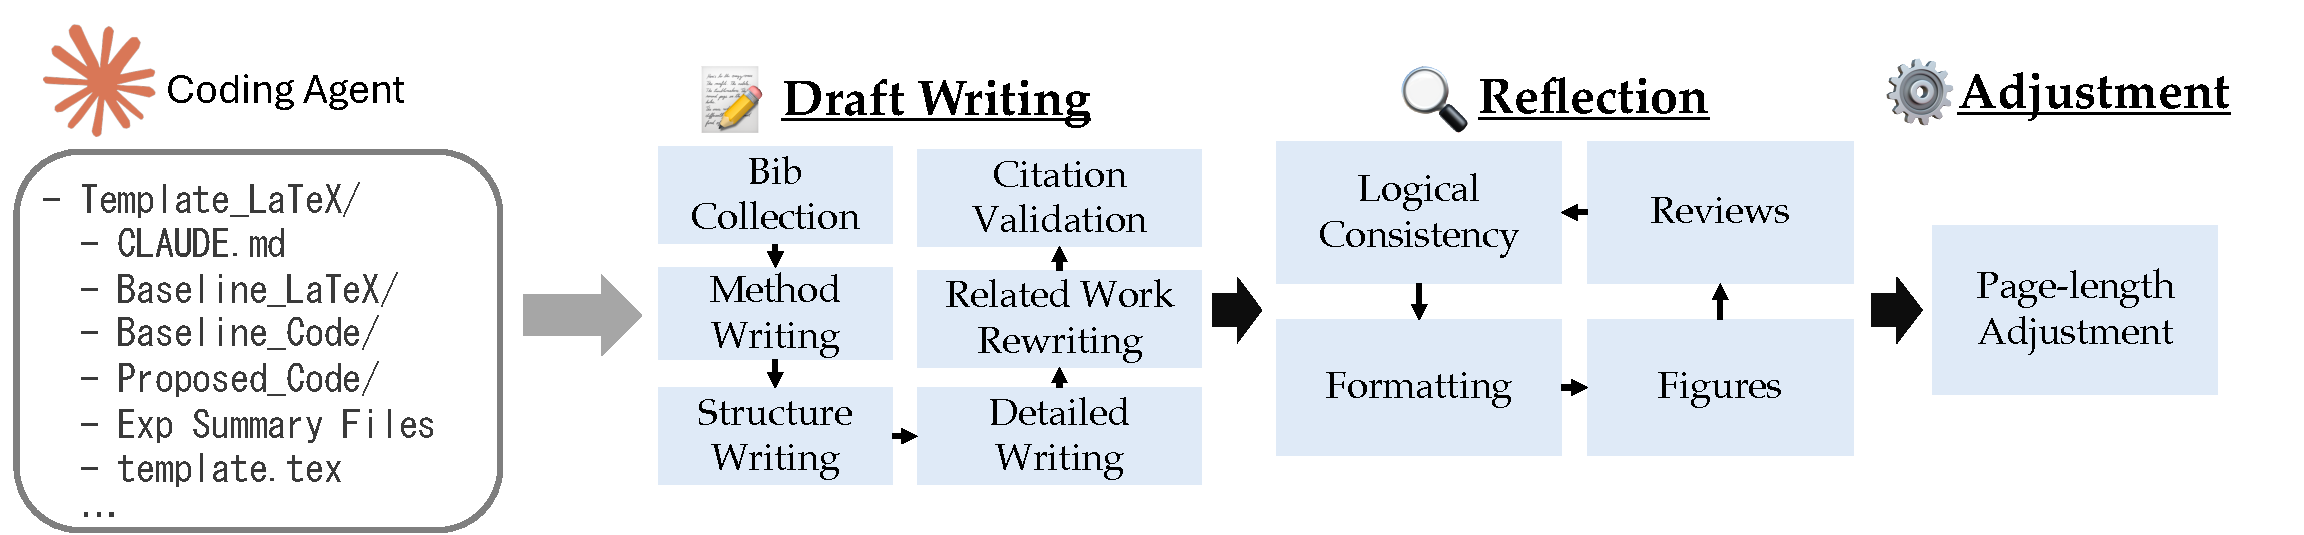
\includegraphics{images/writing_overview.pdf}
    }
    \caption{\textbf{Jr. AI Scientist Workflow for the Writing Phase.} The Writing process consists of three steps: Draft Writing, Reflection, and Adjustment.}
    \label{Fig:writing_workflow}
\vspace{-2em}
\end{figure*}


We primarily used a coding agent (\eg~Claude Code~\citep{claude_code}) as a writing agent for the writing process.
As shown in \Cref{Fig:writing_workflow}, the Writing Phase consists of three stages—Draft Writing, Reflection, and Adjustment.
Below, we describe the resources provided to the writing agent and the details of each stage.

\subsubsection{Preliminary: Resources Provided to Writing Agent}
\textbf{Conference LaTeX Template.}  
We provide the conference LaTeX template to the writing agent.  
We give the Agents4Science template, and the corresponding directory is set as the working directory where the writing agent operates.

\textbf{Instruction Markdown File for the Writing Agent.}  
An instruction file in Markdown format is provided to the writing agent.  
This document defines the overall structure of the paper, outlining how each section should be organized, and offers detailed guidelines on the key points and considerations for writing each part of the manuscript.

\textbf{Baseline LaTeX Files and Code.}  
We provide the writing agent with the baseline LaTeX files and code.  
These resources are mainly used to explain the baseline method in the Method section.

\textbf{Stage 2 Proposed Method Code.}  
The writing agent is also given the Stage 2 code (the proposed method).  
This is primarily referenced in the Method section when explaining the proposed approach.


\textbf{Experiment Summaries for Each Stage.}  
Following the protocol of AI Scientist v2, we provide the writing agent with summarized JSON files containing key experimental results for each stage (\texttt{baseline\_summary.json}, \texttt{improved\_research\_summary.json}, \texttt{component\_ablation\_summary.json}, and \texttt{hyperparam\_ablation\_summary.json}).
These files include essential information such as experimental descriptions, results, and paths for visualization results, which are crucial for the writing agent when writing the experimental results section.  
In addition, for ablation studies, we not only provide the JSON files but also automatically convert them into LaTeX table files (\texttt{component\_ablation\_summary\_table.tex} and \texttt{hyperparam\_ablation\_summary\_table.tex}).  
This conversion has significantly reduced numerical transcription errors in the paper.


The only materials that humans need to prepare for each paper generation are the LaTeX source files and the baseline codebase of the baseline paper. The CLAUDE.md file and the conference LaTeX template are shared across all experiments. The code and experimental files for the proposed methods are automatically generated during the experimental stage. Using these inputs, the AI agent automatically writes all sections and captions in the paper.

\subsubsection{Draft Writing}
As shown in \Cref{Fig:writing_workflow}, the Draft Writing stage follows a multi-step process:
it begins with the collection of BibTeX entries, followed by the writing of the Method section, the generation of the paper structure, and finally the full-paper writing.
Afterward, the system performs a rewrite of the Related Work section and subsequently validates the correctness of citations.
Here, we first explain how we determined the writing order and then describe the detailed procedures for each stage of this workflow.

\textbf{Rationale of Writing Orders.}
Following AI Scientist v2~\citep{yamada2025ai}, we initially generated the entire paper at once, but this resulted in a decline in the quality of the Method section. We therefore adopted a step-by-step writing process to improve overall consistency and quality.
When determining the writing order, we considered it most important for the writing agent to first accurately understand and describe the proposed method, as this understanding serves as the foundation for correctly writing other sections.
Therefore, we instruct the writing agent to focus exclusively on accurately writing the Method section.
In addition, for the paper structure, we followed the approach of AI-Researcher~\citep{tang2025ai} and introduced an intermediate step of summarizing the paper structure, in which the writing agent briefly outlines the content of each section before full-paper generation.
These refinements made it possible to produce more consistent and accurate descriptions throughout a paper.

\textbf{Collection of BibTeX Entries.}
To ensure accurate citation, it is essential to collect a complete and correct set of BibTeX entries.
Following AI Scientist v1~\citep{lu2024ai}, we use the Semantic Scholar API to retrieve BibTeX records.
However, this approach alone often yields an insufficient number of references.
To address this limitation, we adopt a practical strategy commonly used by human researchers: using the baseline paper's BibTeX file as a starting point.
This approach allows the system to gather a sufficient number of references while also can expect correct citation by referring to the baseline's LaTeX source.
Since the baseline's BibTeX file does not include the entry for the baseline reference set, we explicitly add it to the reference set.

\textbf{Method Section Writing.}
For the Method section, we instruct the writing agent to write both a preview of the baseline method and a detailed description of the proposed method. To ensure an accurate description, we refer the writing agent to the LaTeX source of the baseline paper so that it can correctly describe the existing method. We also instruct the writing agent to describe the proposed method based on the Stage 2 implementation code, ensuring that the technical details are precisely reflected in the text. This process yielded more accurate and consistent Method sections.

\textbf{Related Work Section Rewriting.}
To clearly define the position and novelty of the generated research, we instruct the writing agent to rewrite the Related Work section after completing the full paper draft.
Since Jr. AI Scientist aims to update the baseline paper, the Related Work section of the baseline serves as a valuable summary of the research field and provides useful guidance on writing style and structure. Therefore, we instruct the writing agent to refer to the Related Work section in the baseline's LaTeX file when generating its own version.

\textbf{Citation Validation.}
We introduce a citation verification phase at the end of the Draft Writing stage.
Since Jr. AI Scientist updates the baseline paper, it can correctly reuse many of the original citations from the baseline paper.
In this step, the writing agent compares the generated paper with the baseline LaTeX file in terms of the quantity and quality of citations, and is instructed to add missing references and remove inappropriate ones to ensure accurate and consistent citation practices.


\subsubsection{Reflection}
To improve the overall quality of the generated paper, we incorporated multiple reflection processes into our workflow.
We repeat these reflections three times.

\textbf{(1) Feedback Generation and Reflection on Logical Consistency.}
This process aims to enhance the academic reliability of the generated text by producing specific and actionable feedback.
In particular, this process examines several key aspects essential for ensuring the logical soundness of a paper, such as logical consistency, validity of supporting citations, and alignment between experimental results and textual descriptions, and whether each section contains a sufficient amount of content.
We first instruct the writing agent to generate feedback regarding the above aspects, and then use it to revise the draft based on that feedback. This process encourages the generation of more logically coherent and trustworthy papers.

\textbf{(2) Reflection on Formatting and Presentation.}
Following AI Scientist v2~\citep{yamada2025ai}, we also introduce a reflection phase focused on formatting and presentation quality.
In this phase, the writing agent generates feedback such as:
``Are there any LaTeX syntax errors or style violations we can fix? Refer to the chktex output below'', or
``Are there short sections (one or two sentences) that could be combined into a single paragraph?''
This process helps produce a final draft that is well-formatted and stylistically consistent.


\textbf{(3) Feedback Generation and Reflection on Figures.}
Following AI Scientist v2~\citep{yamada2025ai}, we perform figure-level reflection in the refinement stages by integrating a Large Multimodal Model (LMM)-based feedback mechanism.
This process aims to improve the quality, clarity, and alignment of generated figures, captions, and their corresponding textual interpretations.
Specifically, the LMM is used to identify figures that are uninformative or make little contribution to the paper's scientific value, and such figures are either removed or moved to the Appendix.
This ensures that all figures presented in the main paper contain adequate informational value.
To achieve this, we provide the LMM with the paper's abstract, figure captions, and figure images to generate targeted feedback, which is then used to guide the reflection and revision process.

\textbf{(4) Feedback Generation and Reflection from AI Reviews.}
Following CycleResearcher~\citep{weng2024cycleresearcher}, we adopt a review-based reflection, where the system improves its manuscript based on reviewer feedback.
In this step, the writing agent revises the generated paper according to reviewer comments such as ``the Method section is unclear'', ``important parameter details are missing'', or ``the writing is overly verbose''.
For generating such feedback, we employ  AI reviewers in AI Scientist v1 (text-only evaluation) and v2 (evaluation including figures).
These AI reviewers use GPT-4o~\citep{gpt4o} and are prompted to evaluate papers in the official NeurIPS review format.

% \miyai{sakanaのv2もReflectionがあったり、CircularResearcherもReflectionがあったりするので、完全に正しいものであるとは考えないように。}
% \otonari{CycleResearcherも査読フィードバックをしているようなので新規性の主張が厳しい気がした。}

\subsubsection{Adjustment: Page-length Adjustment}
We also introduced a new design to the page-length adjustment process. In AI Scientist v2~\citep{yamada2025ai}, when the generated paper exceeded the predefined page limit, the system attempted to adjust the length within a single LLM call. However, this approach often resulted in over-trimming, causing the paper to become significantly shorter than the target length. To address this issue, our method performs iterative and gradual page-length reduction until the manuscript reaches the target length, thereby improving the stability of page adjustment.
As a result, the final papers consistently fell within $\pm$ 1 page of the specified page limit.
We set the page layout to 8 pages.